\documentclass[a4paper,11pt]{article}%

\usepackage{fullpage}%
\usepackage[T1]{fontenc}%
\usepackage[utf8]{inputenc}%
\usepackage[main=francais,english]{babel}% % Adjust the main language

\usepackage{graphicx}%
\usepackage{url}%
\usepackage{abstract}%

\usepackage{amsmath}%
\usepackage{subfig}%

\usepackage{newpxtext, newpxmath}

\usepackage{listings}%

\lstset{%
  basicstyle=\sffamily,%
  columns=fullflexible,%
  language=R,%       % Adjust according to your current language
  frame=lb,%
  frameround=fftf,%
  literate=
  {á}{{\'a}}1 {é}{{\'e}}1 {í}{{\'i}}1 {ó}{{\'o}}1 {ú}{{\'u}}1
  {Á}{{\'A}}1 {É}{{\'E}}1 {Í}{{\'I}}1 {Ó}{{\'O}}1 {Ú}{{\'U}}1
  {à}{{\`a}}1 {è}{{\`e}}1 {ì}{{\`i}}1 {ò}{{\`o}}1 {ù}{{\`u}}1
  {À}{{\`A}}1 {È}{{\'E}}1 {Ì}{{\`I}}1 {Ò}{{\`O}}1 {Ù}{{\`U}}1
  {ä}{{\"a}}1 {ë}{{\"e}}1 {ï}{{\"i}}1 {ö}{{\"o}}1 {ü}{{\"u}}1
  {Ä}{{\"A}}1 {Ë}{{\"E}}1 {Ï}{{\"I}}1 {Ö}{{\"O}}1 {Ü}{{\"U}}1
  {â}{{\^a}}1 {ê}{{\^e}}1 {î}{{\^i}}1 {ô}{{\^o}}1 {û}{{\^u}}1
  {Â}{{\^A}}1 {Ê}{{\^E}}1 {Î}{{\^I}}1 {Ô}{{\^O}}1 {Û}{{\^U}}1
  {œ}{{\oe}}1 {Œ}{{\OE}}1 {æ}{{\ae}}1 {Æ}{{\AE}}1 {ß}{{\ss}}1
  {ű}{{\H{u}}}1 {Ű}{{\H{U}}}1 {ő}{{\H{o}}}1 {Ő}{{\H{O}}}1
  {ç}{{\c c}}1 {Ç}{{\c C}}1 {ø}{{\o}}1 {å}{{\r a}}1 {Å}{{\r A}}1
  {€}{{\euro}}1 {£}{{\pounds}}1 {«}{{\guillemotleft}}1
  {»}{{\guillemotright}}1 {ñ}{{\~n}}1 {Ñ}{{\~N}}1 {¿}{{?`}}1,%
}%

\parskip=0.5\baselineskip

\sloppy

\begin{document}

\title{Maths 2: Devoir Maison de statistiques appliquées}

\author{Marco Freire \and Clément Legrand-Duchesne}

\date{25 mars 2018}

\maketitle

\begin{abstract}
  
  \begin{description}
    
  \item[Mots-clefs:] 
      
  \item[Classification ACM:] 
  \end{description}
\end{abstract}

\renewcommand{\contentsname}{Plan}
\tableofcontents

\section{Description du jeu de données}
Le jeu de données fournis contient les mesures de la qualité des
programmes couramment utilisés par les biologistes. Seize programmes
sont ainsi examinés, selon des critères tels que le nombre de lignes ou
de blocs dupliqués, le nombre et le type de warning lors de la
compilation ou encore le statut donné par valgrind sur la gestion
mémoire.

Un premier graphique nous permet de compter le nombre de programme
écrit dans chaque langage du jeu de donnée (figure \ref{fig:prog_lang}).

Nous avons ensuite décider de représenter le nombre de lignes de codes
par programme (figure \ref{fig:lin_prog}). Afin que la représentation
soit plus lisible, nous avons utilisé la commande \lstinline{order}
pour ordonner les colonnes par ordres décroissants de valeurs. De
plus, nous avons affiché les noms des programmes en vertical, afin
d'améliorer la lisibilité (grâce à l'argument \lstinline{las = 2} de
\lstinline{barplot}).

De même, nous avons créer un histogrammes contenant le nombre de blocs
dupliqués par programme (figure \ref{fig:dbl_prog}). Il est nécessaire
de faire attention à ne pas prendre en compte les programmes pour
lesquels cette valeur n'est pas renseignée (c'est le cas de \emph{FDPPDIV}
par exemple).

Enfin, nous avons généré un dernier graphique affichant le nombre de
programmes par domaine (figure \ref{fig:prog_dom}).

\begin{figure}[!h]
  \minipage{0.48\textwidth}
  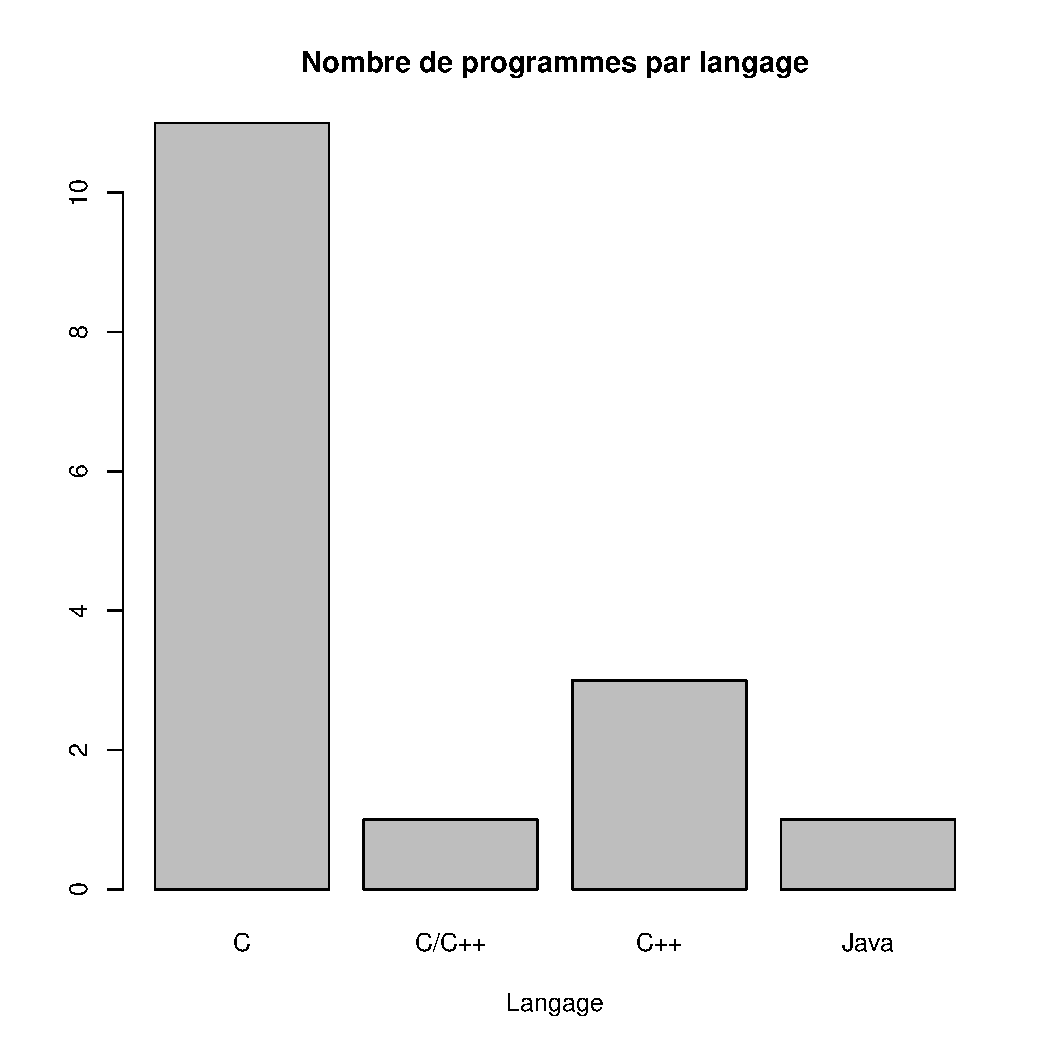
\includegraphics[width=\linewidth]{figures/prog_lang.pdf}
  \caption{}\label{fig:prog_lang}
  \endminipage\hfill
  \minipage{0.48\textwidth}
  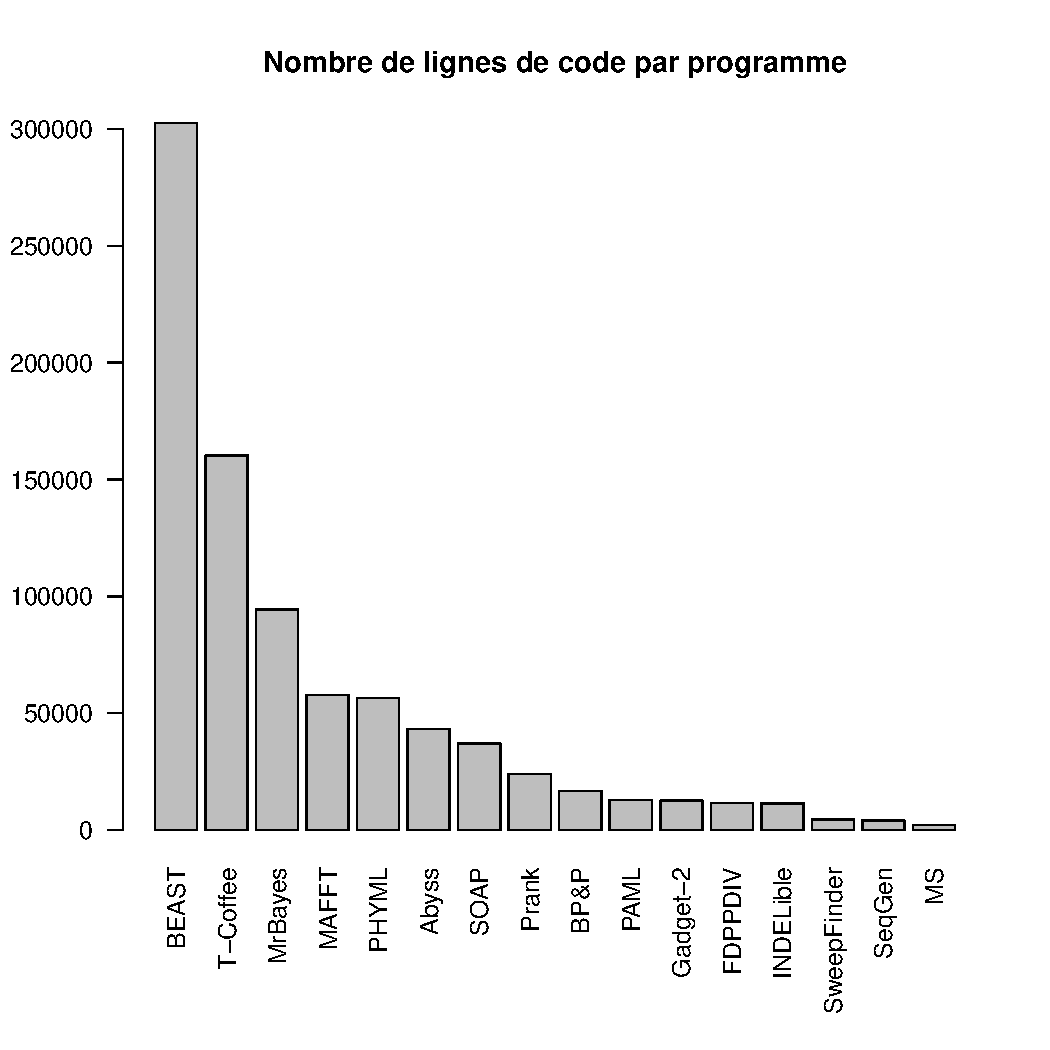
\includegraphics[width=\linewidth]{figures/lin_prog.pdf}
  \caption{}\label{fig:lin_prog}
  \endminipage\hfill
  \minipage{0.48\textwidth}
  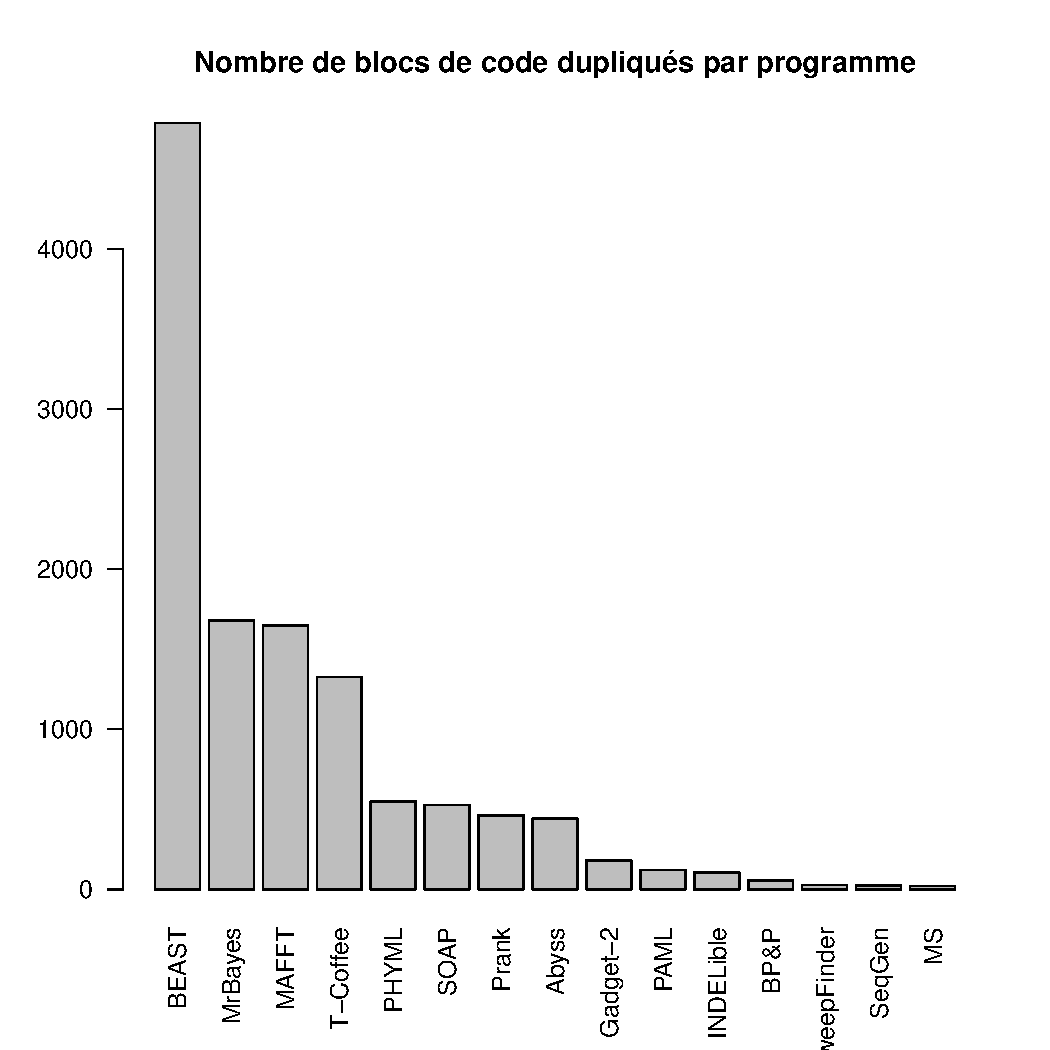
\includegraphics[width=\linewidth]{figures/dbl_prog.pdf}
  \caption{}\label{fig:dbl_prog}
  \endminipage\hfill
  \minipage{0.48\textwidth}
  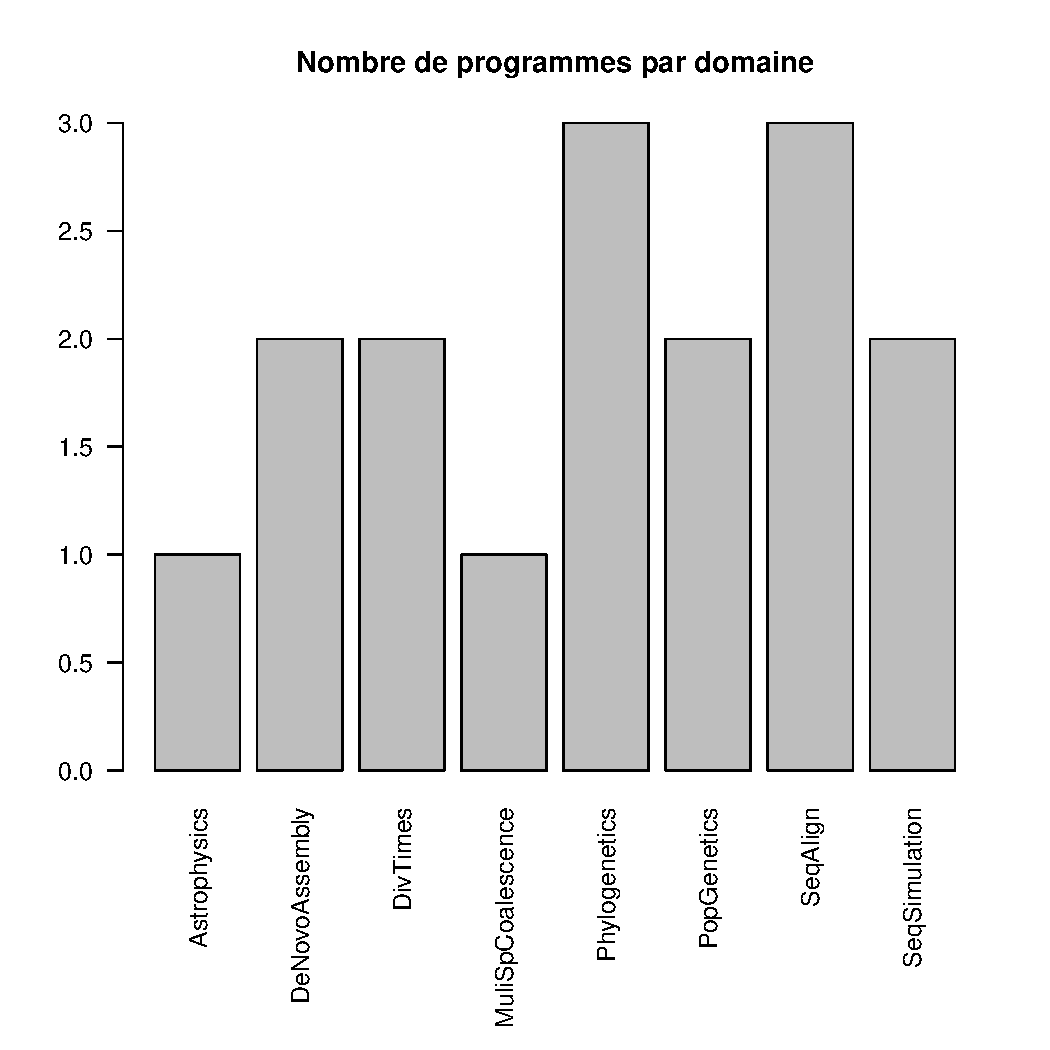
\includegraphics[width=\linewidth]{figures/prog_dom.pdf}
  \caption{}\label{fig:prog_dom}
  \endminipage\hfill
\end{figure}

\section{Pourcentage de lignes de code dupliquées}
Afin de calculer le pourcentage de ligne dupliquées, nous avons créé
une nouvelle table, contenant les noms des programmes, leurs
dommaines, les langages dans lesquels ils ont été écrits et leurs
nombres de lignes dupliquées (figure \ref{fig:dlin_prog}) ainsi que
leurs nombres de lignes totales. Nous avons enlevé de cette nouvelle
table de données les programmes pour ayant un champs non renseigné (à
l'aide de la commande \emph{na.omit}). Nous avons ensuite rajouté une
colonne à celle ci contenant les pourcentages de lignes de codes
dupliquées, avant de créer un histogrammes de ces pourcentages pour
chaque programme, ordonné par ordre décroissant (figure
\ref{fig:pdlin_prog}).

\begin{figure}[!h]
  \minipage{0.48\textwidth}
  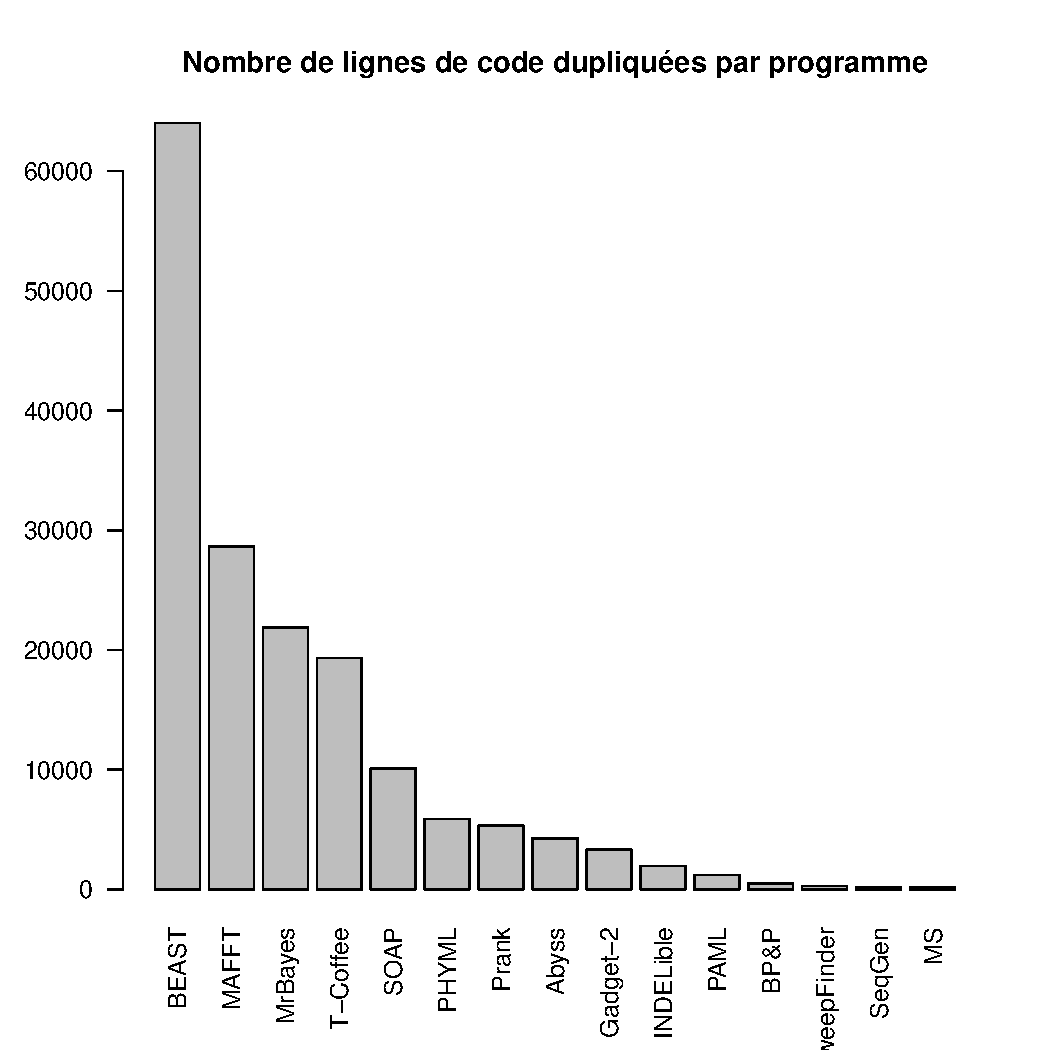
\includegraphics[width=\linewidth]{figures/dlin_prog.pdf}
  \caption{}\label{fig:dlin_prog}
  \endminipage\hfill
  \minipage{0.48\textwidth}
  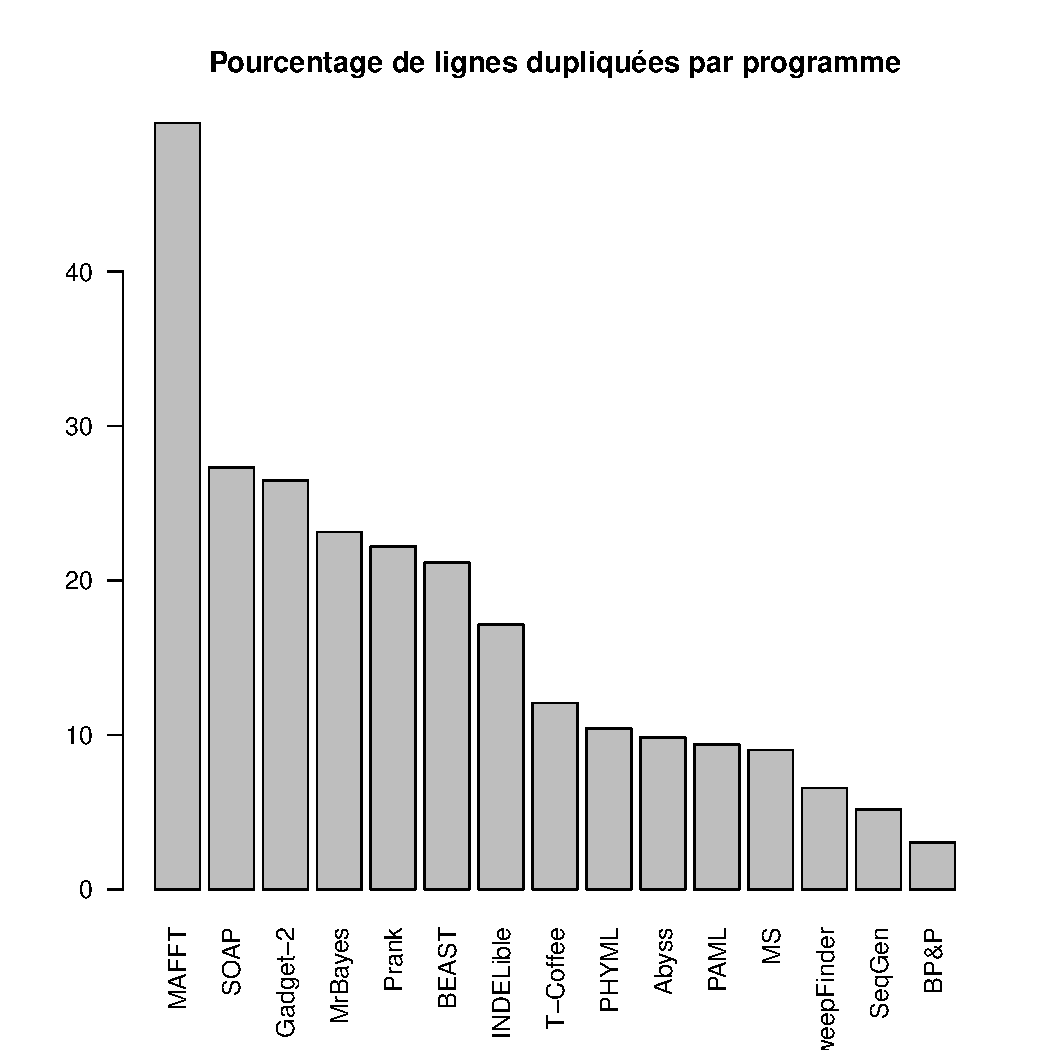
\includegraphics[width=\linewidth]{figures/pdlin_prog.pdf}
  \caption{}\label{fig:pdlin_prog}
  \endminipage\hfill
\end{figure}

\section*{Annexe}
\lstinputlisting{../fusion.R}

\end{document}
